% ==============================================================================
% PAGE 17: 2) RECEIVER (Numbered Page 9)
% ==============================================================================
\subsubsection*{2) RECEIVER}

\begin{center}
  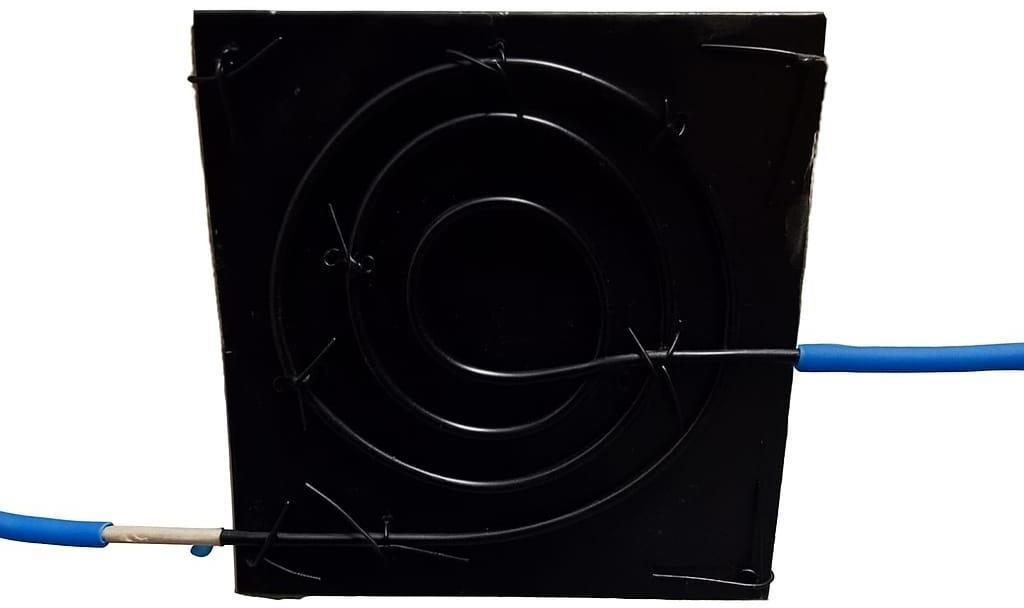
\includegraphics[width=90mm]{figures/fig2_receiver.jpg}
\end{center}

\vspace{3mm}
\noindent
\begin{spacing}{1.2}
{\fontsize{10.2}{14.5}\selectfont
In this project, the receiver plays a vital role in absorbing concentrated solar radiation and converting it into thermal energy. The receiver is fabricated from a copper coil with an internal diameter of 3~mm, selected for its excellent thermal conductivity and corrosion resistance. Copper is an ideal material for solar thermal systems as it ensures rapid heat transfer from the concentrated sunlight to the working fluid circulating inside the coil.\\[3mm]
The receiver coil is positioned precisely at the focal point of the parabolic concentrator, where maximum solar energy is focused.\\[3mm]
To enhance heat absorption and minimize reflective losses, the copper coil is coated with matte black heat-resistant paint. The black surface increases the absorptivity of the receiver, allowing it to capture a greater portion of incident solar radiation. The small internal diameter ensures a higher rate of heat transfer to the flowing water, enabling quick temperature rise and even steam generation under continuous solar exposure. This receiver design ensures efficient energy utilization and contributes significantly to the overall performance and thermal efficiency of the solar water heater and steam generator system.
}
\end{spacing}
\clearpage
